\documentclass[11pt, oneside]{article}   	% use "amsart" instead of "article" for AMSLaTeX format
\usepackage{geometry}                		% See geometry.pdf to learn the layout options. There are lots.
\geometry{letterpaper}                   		% ... or a4paper or a5paper or ... 
%\geometry{landscape}                		% Activate for rotated page geometry
%\usepackage[parfill]{parskip}    		% Activate to begin paragraphs with an empty line rather than an indent
\usepackage{graphicx}				% Use pdf, png, jpg, or eps§ with pdflatex; use eps in DVI mode
								% TeX will automatically convert eps --> pdf in pdflatex		
\usepackage{amssymb}
\usepackage{amsmath}
\usepackage{float}
%SetFonts

\usepackage[utf8]{inputenc}
\newcommand{\Var}{\operatorname{Var}}
% Default fixed font does not support bold face
\DeclareFixedFont{\ttb}{T1}{txtt}{bx}{n}{12} % for bold
\DeclareFixedFont{\ttm}{T1}{txtt}{m}{n}{12}  % for normal

% Custom colors
\usepackage{color}
\definecolor{deepblue}{rgb}{0,0,0.5}
\definecolor{deepred}{rgb}{0.6,0,0}
\definecolor{deepgreen}{rgb}{0,0.5,0}

\usepackage{listings}

% Python style for highlighting
\newcommand\pythonstyle{\lstset{
language=Python,
basicstyle=\ttm,
otherkeywords={self},             % Add keywords here
keywordstyle=\ttb\color{deepblue},
emph={MyClass,__init__},          % Custom highlighting
emphstyle=\ttb\color{deepred},    % Custom highlighting style
stringstyle=\color{deepgreen},
frame=tb,                         % Any extra options here
showstringspaces=false            % 
}}


% Python environment
\lstnewenvironment{python}[1][]
{
\pythonstyle
\lstset{#1}
}
{}

% Python for external files
\newcommand\pythonexternal[2][]{{
\pythonstyle
\lstinputlisting[#1]{#2}}}

% Python for inline
\newcommand\pythoninline[1]{{\pythonstyle\lstinline!#1!}}

\title{Mixed statistical and signal processing method for predictive maintenance: A use case for two types of bearing defect detection}
\author{Yapi Donatien Achou}
%\date{}							% Activate to display a given date or no date

\begin{document}
\maketitle
\begin{figure}[H] %  figure placement: here, top, bottom, or page
   \centering
   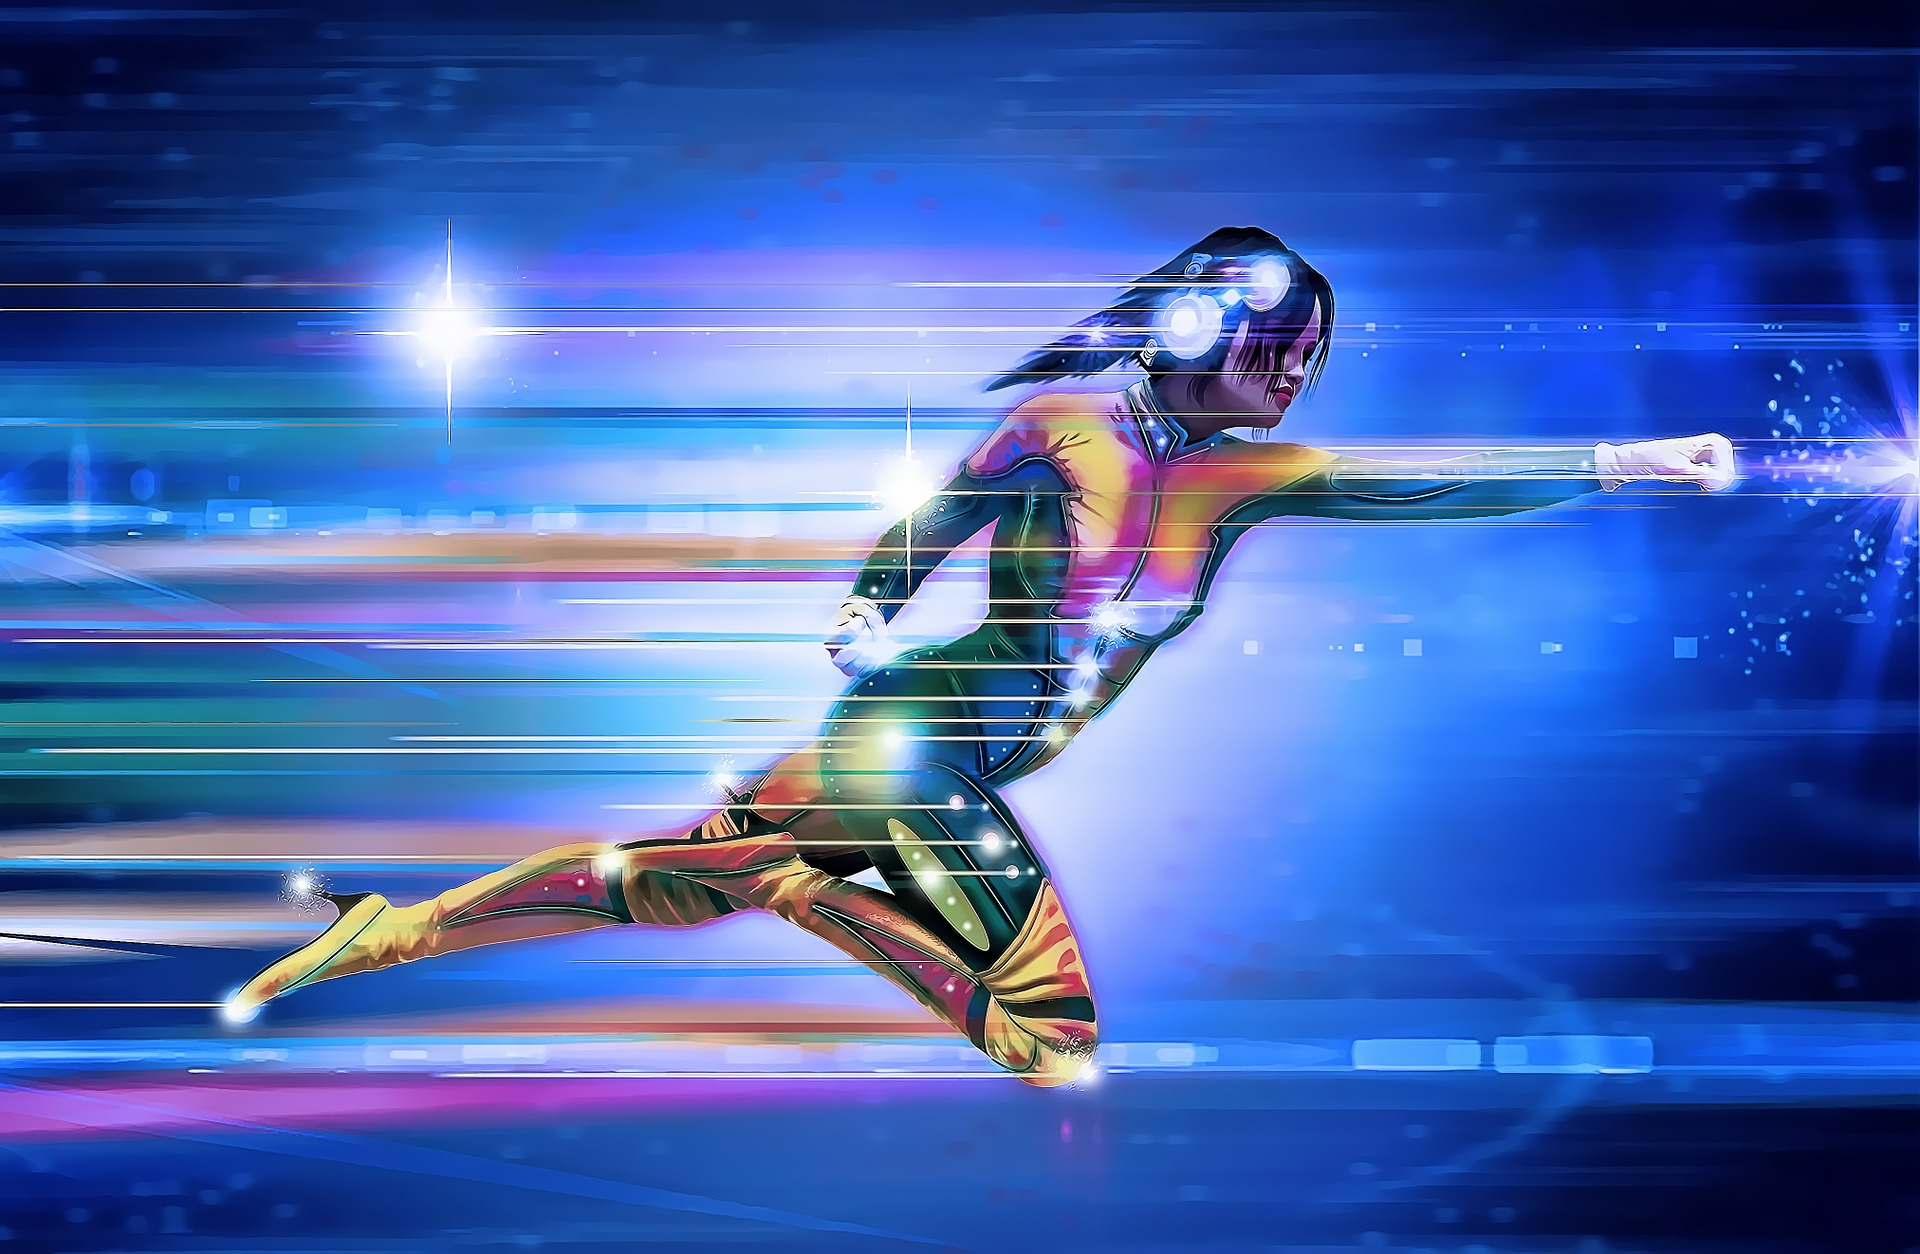
\includegraphics[width=5in]{front4} 
   \caption{}
   \label{fig:example}
\end{figure}
\section{Introduction}
Predictive maintenance can be defined as a maintenance philosophy with a set of methods used to predict and prevent machine failure in order to avoid unexpected downtime. This maintenance philosophy when correctly implemented, increases machine life time, and reduces maintenance cost [referecne].
\begin{flushleft}
In rotating machines, more than 40 $\%$ of machine malfunction can be attributed to bearing defect [references]. 
\end{flushleft}
\begin{figure}[H] %  figure placement: here, top, bottom, or page
   \centering
   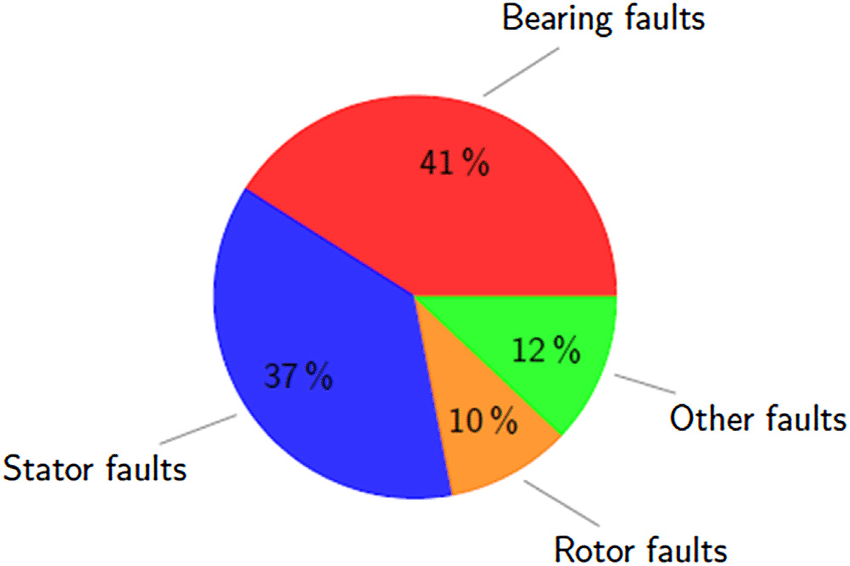
\includegraphics[width=5in]{pie.png} 
   \caption{Defect statistic, taken from [reference]}
   \label{fig:pie}
\end{figure}
In this post I will present a signal processing method , a statistical and a mixed method to detect bearing defect.

\section{Defining the use case}
\begin{figure}[H] %  figure placement: here, top, bottom, or page
   \centering
   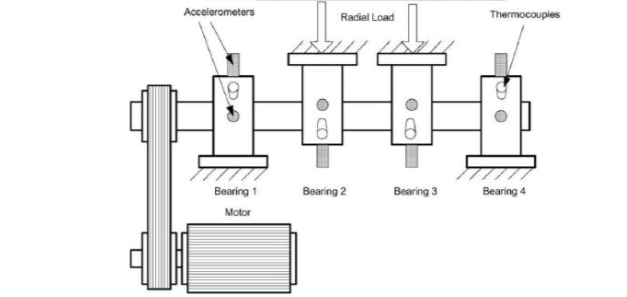
\includegraphics[width=4in]{experiment} 
   \caption{Experimental set up}
   \label{fig:exp}
\end{figure}
The data used in this use case was generated by the Intelligence Maintenance system (IMS) [link to the IMS].
Three separate experiments involving four bearings were performed on a motor. In each experiment, a 1-second vibration signal snapshots was recorded every 10 minutes, for a specified time. Each vibrational signal sample consists of 20 480 data points with sampling rate of 20 000 Hz.
In this post I will be using the first and the second experiment data [available here (give a link to the data)].



%%%%%%%%%%%%%%%%%%%%%%%%%%%%%%%%%%%%%%%%%%%%%%%%%%%%%%%%%%%%%%%%%%%%%%%%%%%%%%%%%%%%
%%%%%%%%%%%%%%%%%%%%%%%%%%%%%%%%%%%%%%%%%%%%%%%%%%%%%%%%%%%%%%%%%%%%%%%%%%%%%%%%%%%%
%%%%%%%%%%%%%%%%%%%%%%%%%%%%%%%%%%%%%%%%%%%%%%%%%%%%%%%%%%%%%%%%%%%%%%%%%%%%%%%%%%%%

\section{Signal processing approach}
\begin{figure}[H] %  figure placement: here, top, bottom, or page
   \centering
   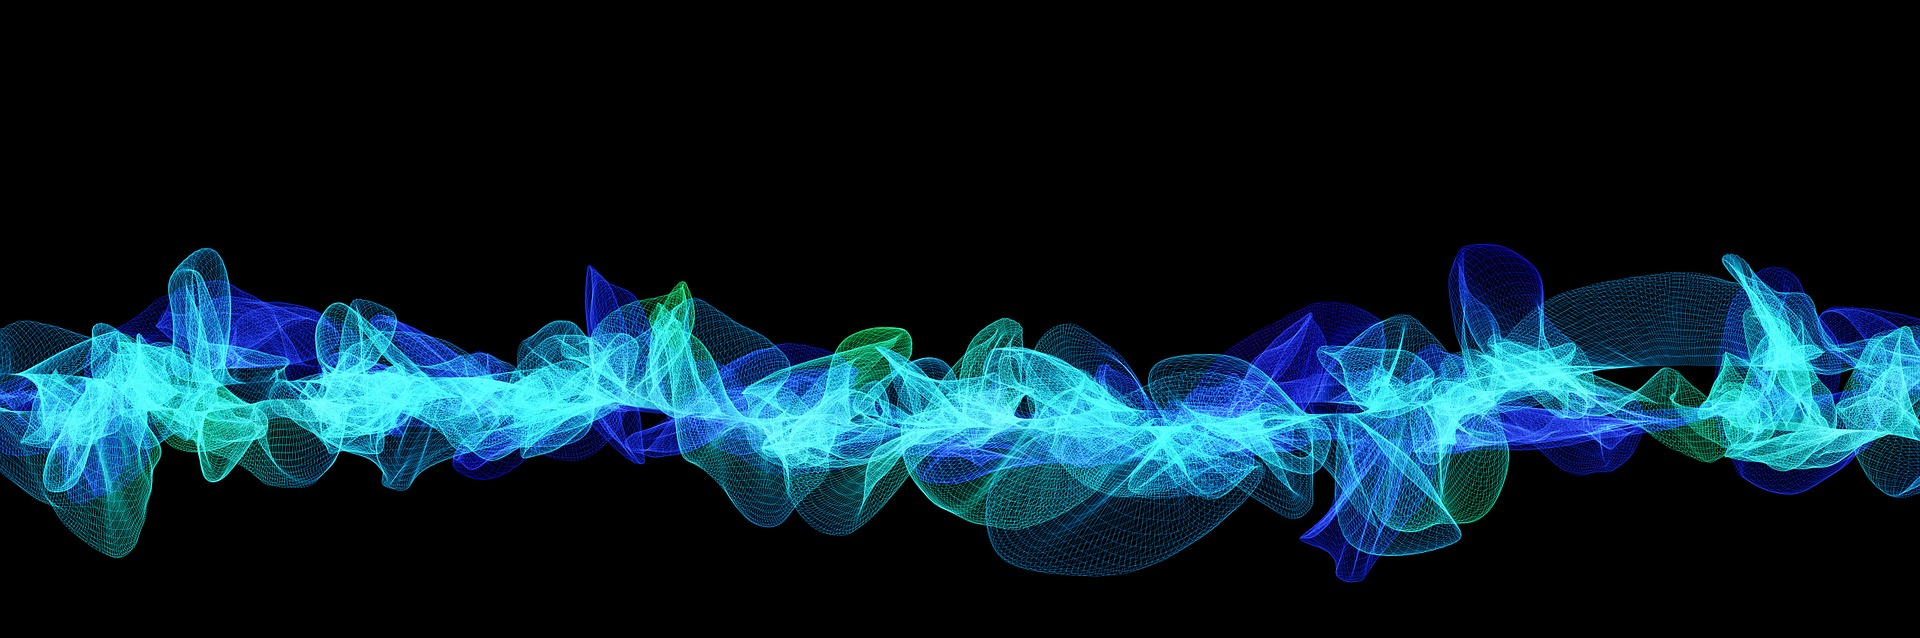
\includegraphics[width=4in]{vibration} 
   \caption{}
   \label{fig:example}
\end{figure}
In this approach we use the old goody Fourier transform. Firstly, we need the defect frequency for the outer race defect and the inner race defect. The bearing type used are Rexnor ZA-2115. For this type of bearing, the constant defect frequency (cdf) for ball pass frequency outer race defect is 0.1182 and the constant defect frequency for ball pass frequency inner race defect is 0.1484 [reference]. According to Rexnord product engineering group [reference, last page], to find the defect frequency in Hz we multiply the constant defect frequency (cdf) by the rotational speed of the bearing ( here 2000 RPM), to find the defect frequency in Hz. Note that the defect frequency is computed from the geometry of the bearing, which means that for a specific bearing, this is a constant value.
\begin{figure}[H] %  figure placement: here, top, bottom, or page
   \centering
   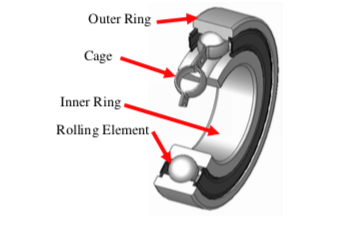
\includegraphics[width=4in]{bearing.png} 
   \caption{}
   \label{fig:example}
\end{figure}
\begin{flushleft}
\begin{figure}[H] %  figure placement: here, top, bottom, or page
   \centering
   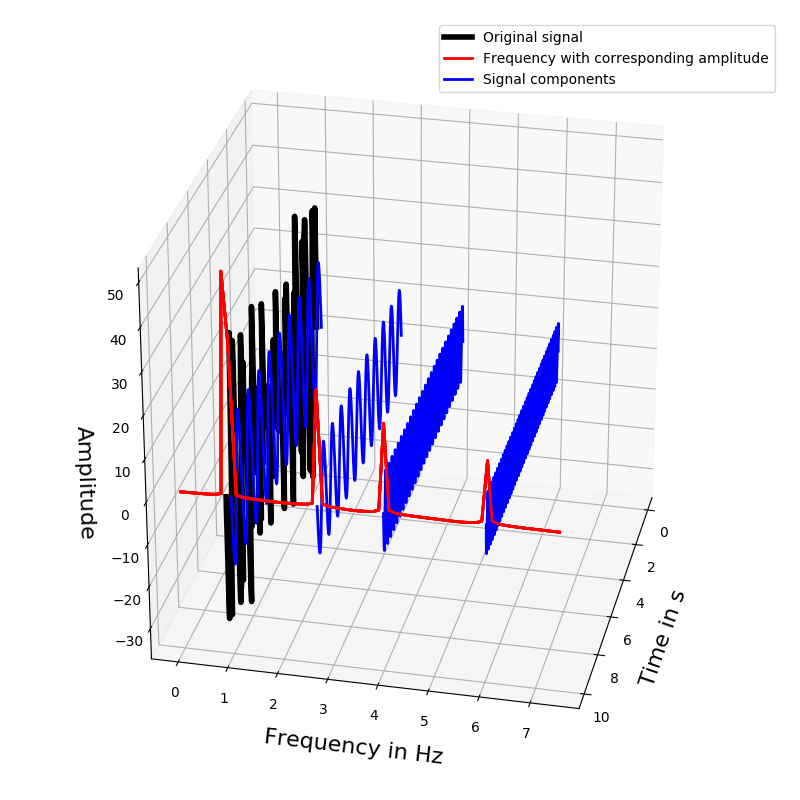
\includegraphics[width=4in]{decomposition} 
   \caption{example caption}
   \label{fig:example}
\end{figure}

Next, we compute the envelop spectrum for each vibration signal by using the FFT method (Fast Fourier Transform). The envelop spectrum is used to detect early sign of failure. Recall that a vibration signal can be decomposed into its sub components, where each  sub component 
is characterised by its frequency and its amplitude. Early sign of failure can be seen in the high frequency low amplitude sub component. As the failure becomes more pronounced, it becomes visible in the low frequency high amplitude sub component.
\end{flushleft}

\begin{figure}[H] %  figure placement: here, top, bottom, or page
   \centering
   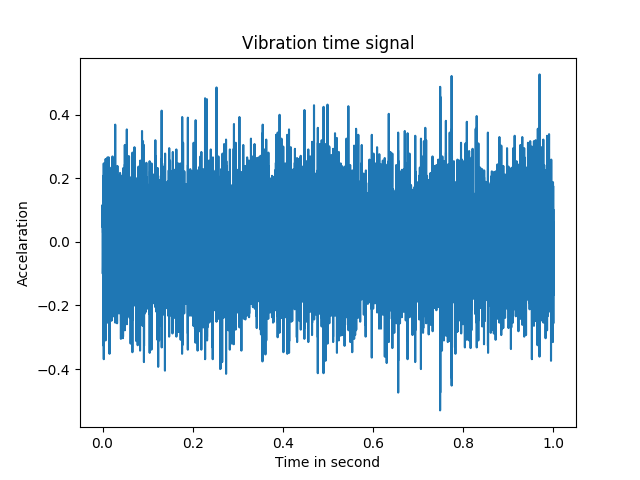
\includegraphics[width=4in]{time-signal.png} 
   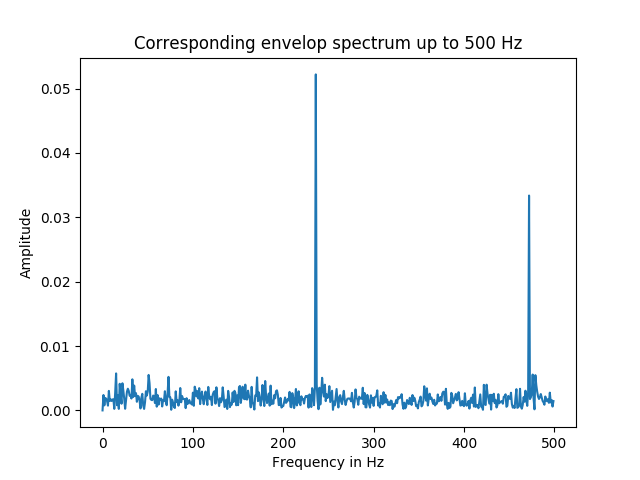
\includegraphics[width=4in]{spectrum.png} 
      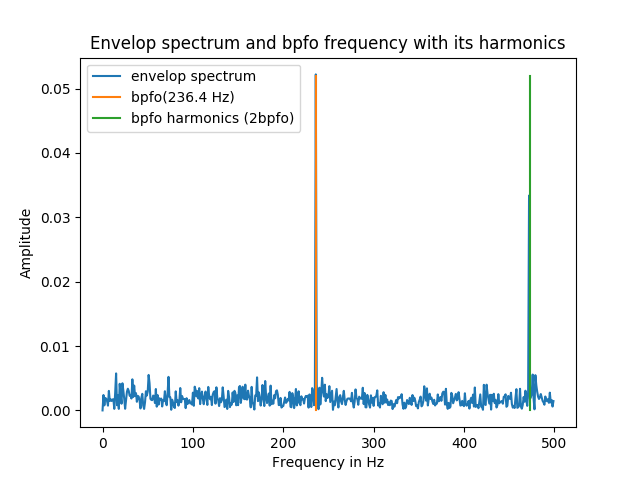
\includegraphics[width=4in]{fault.png} 
   \caption{Vibration time signal}
   \label{fig:signal}
\end{figure}
By computing the envelop spectrum for each time signal and extracting the amplitude of a defect frequency we can visualise the severity of a defect

\begin{figure}[H] %  figure placement: here, top, bottom, or page
   \centering
   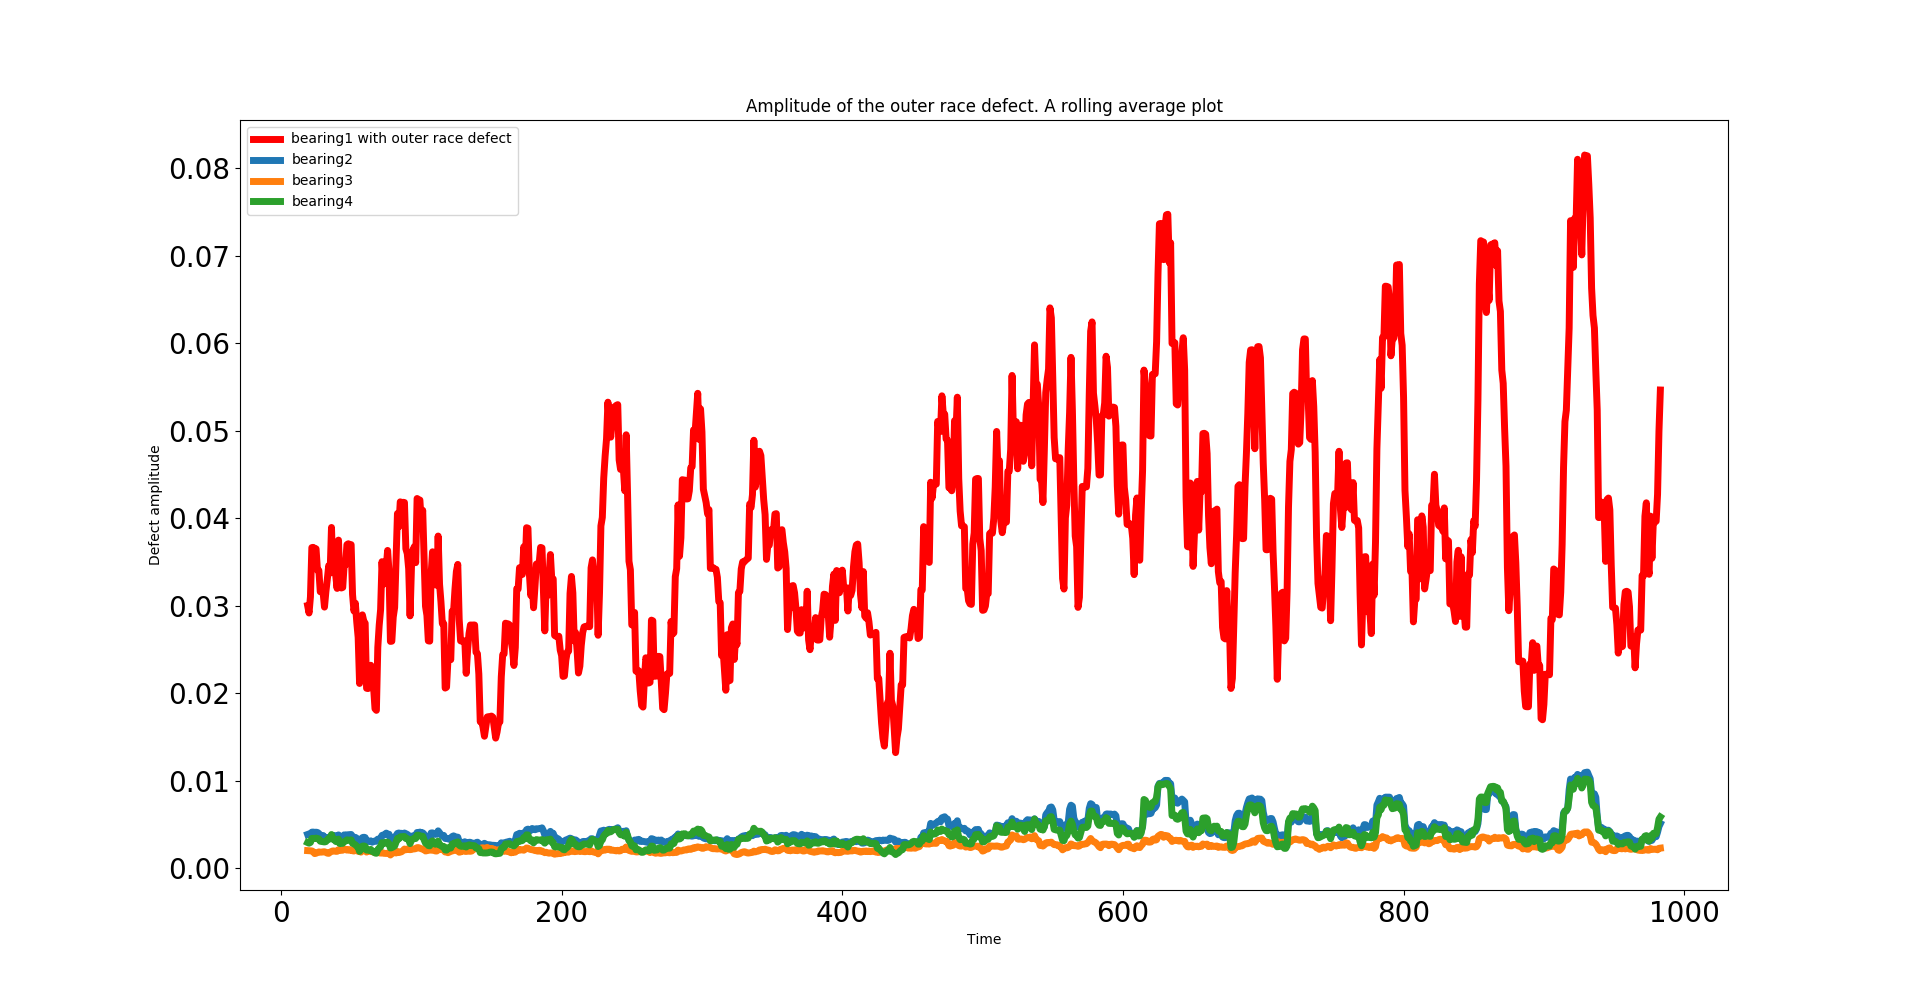
\includegraphics[width=7in]{signal_processing_method_bpfo} 
   \caption{Ball pass frequency outer race detection}
   \label{fig:example}
\end{figure}

\begin{figure}[H] %  figure placement: here, top, bottom, or page
   \centering
   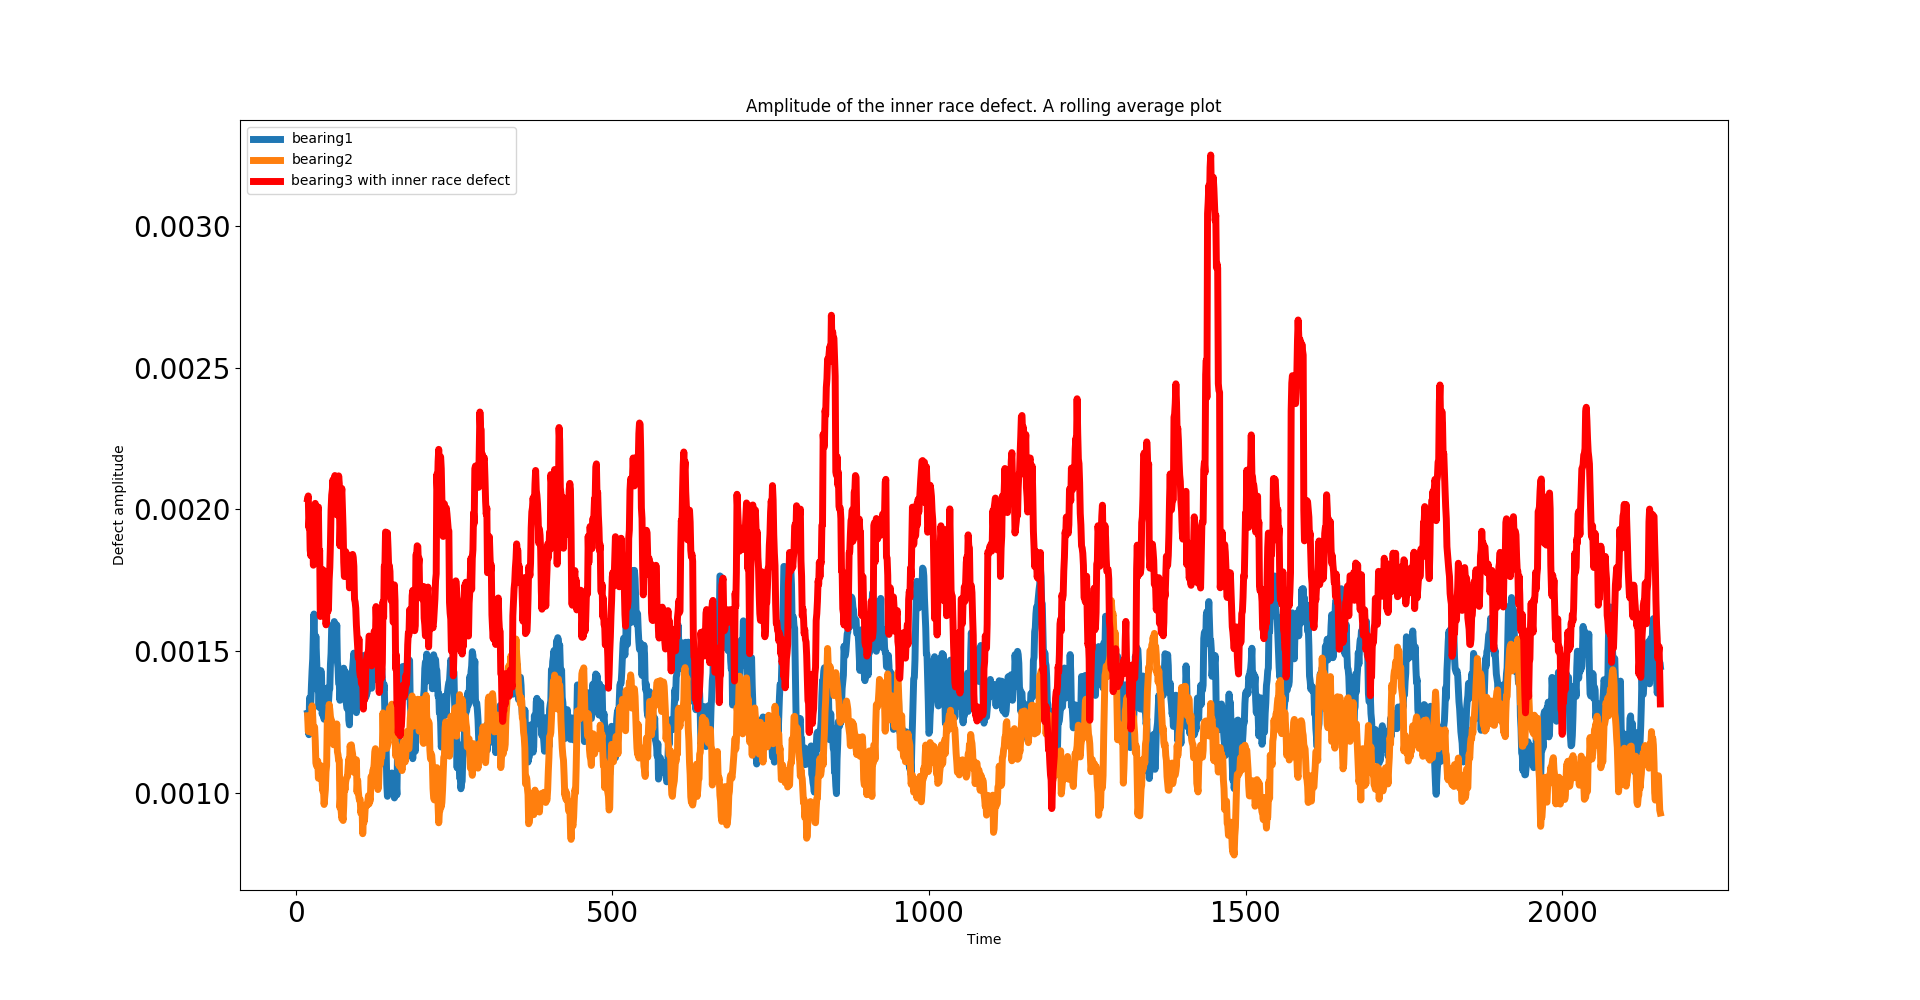
\includegraphics[width=7in]{signal_processing_method_bpfi} 
   \caption{Ball pass frequency inner race detection}
   \label{fig:example}
\end{figure}


%%%%%%%%%%%%%%%%%%%%%%%%%%%%%%%%%%%%%%%%%%%%%%%%%%%%%%%%%%%%%%%%%%%%%%%%%%%%%%%%%%%%
%%%%%%%%%%%%%%%%%%%%%%%%%%%%%%%%%%%%%%%%%%%%%%%%%%%%%%%%%%%%%%%%%%%%%%%%%%%%%%%%%%%%
%%%%%%%%%%%%%%%%%%%%%%%%%%%%%%%%%%%%%%%%%%%%%%%%%%%%%%%%%%%%%%%%%%%%%%%%%%%%%%%%%%%%
\section{Statistical approach: dissimilarity measure}
In this approach we compute the dissimilarity between each sample. Let $X_{i}$ and $X_{j}$ be two samples from the same distribution. Then the Mahalanobis distance between the two random variables with corresponding covariance matrix $S$ and inverse $S^{-1}$ is given by
\begin{equation}
d(X_{i}, X_{j}) = \sqrt{  \left(  X_{i}- X_{j} \right)^{T}S^{-1} \left(  X_{i}- X_{j} \right)    }
\end{equation}
The Mahalobis distance then gives the dissimilarity between the two samples $X_{i}$ and $X_{j}$.
\begin{flushleft}
Our dissimilarity measure is inspired by the Mahalanobis distance. Rather then using $X_{i}-X_{j}$ we will form a vector $\left(\Var[X_{i}], \Var[X_{j}]\right)$ where $\Var[X_{i}]$ and$\Var[X_{i}]$ are the variance of sample $X_{i}$ and $X_{j}$ respectively. With this change the new dissimilarity measure is given by 
\begin{equation}
d(Z, Y) =  \left(  \Var[Z], \Var[Y] \right)^{T}S^{-1} \left( \Var[Z], \Var[Y] \right]) .
\end{equation}
\end{flushleft}
Once we have a way to measure the dissimilarity between samples, we set a reference sample $X_{0}$ which represents a sample with no defect. Afterwards,  we compute the dissimilarity between $X_{0}$ and subsequent samples for each bearing.
We can implement the above formula in python:

\begin{python}
def dissimilarity_measure(u,v):
	#inverse of the covariance matrix
	U=np.array([u,v])
	covariance=np.cov(U)
	cov_inv=np.linal.inv(covariance)
	#dissimilarity between u and v
	V=np.array(list(map(lambda w: np.var(w),[u,v]))).reshape(-1,1).T
	d=np.matmul(np.matmul(V,cov_inv), V.T)
	return d
\end{python}
\begin{figure}[H] %  figure placement: here, top, bottom, or page
   \centering
   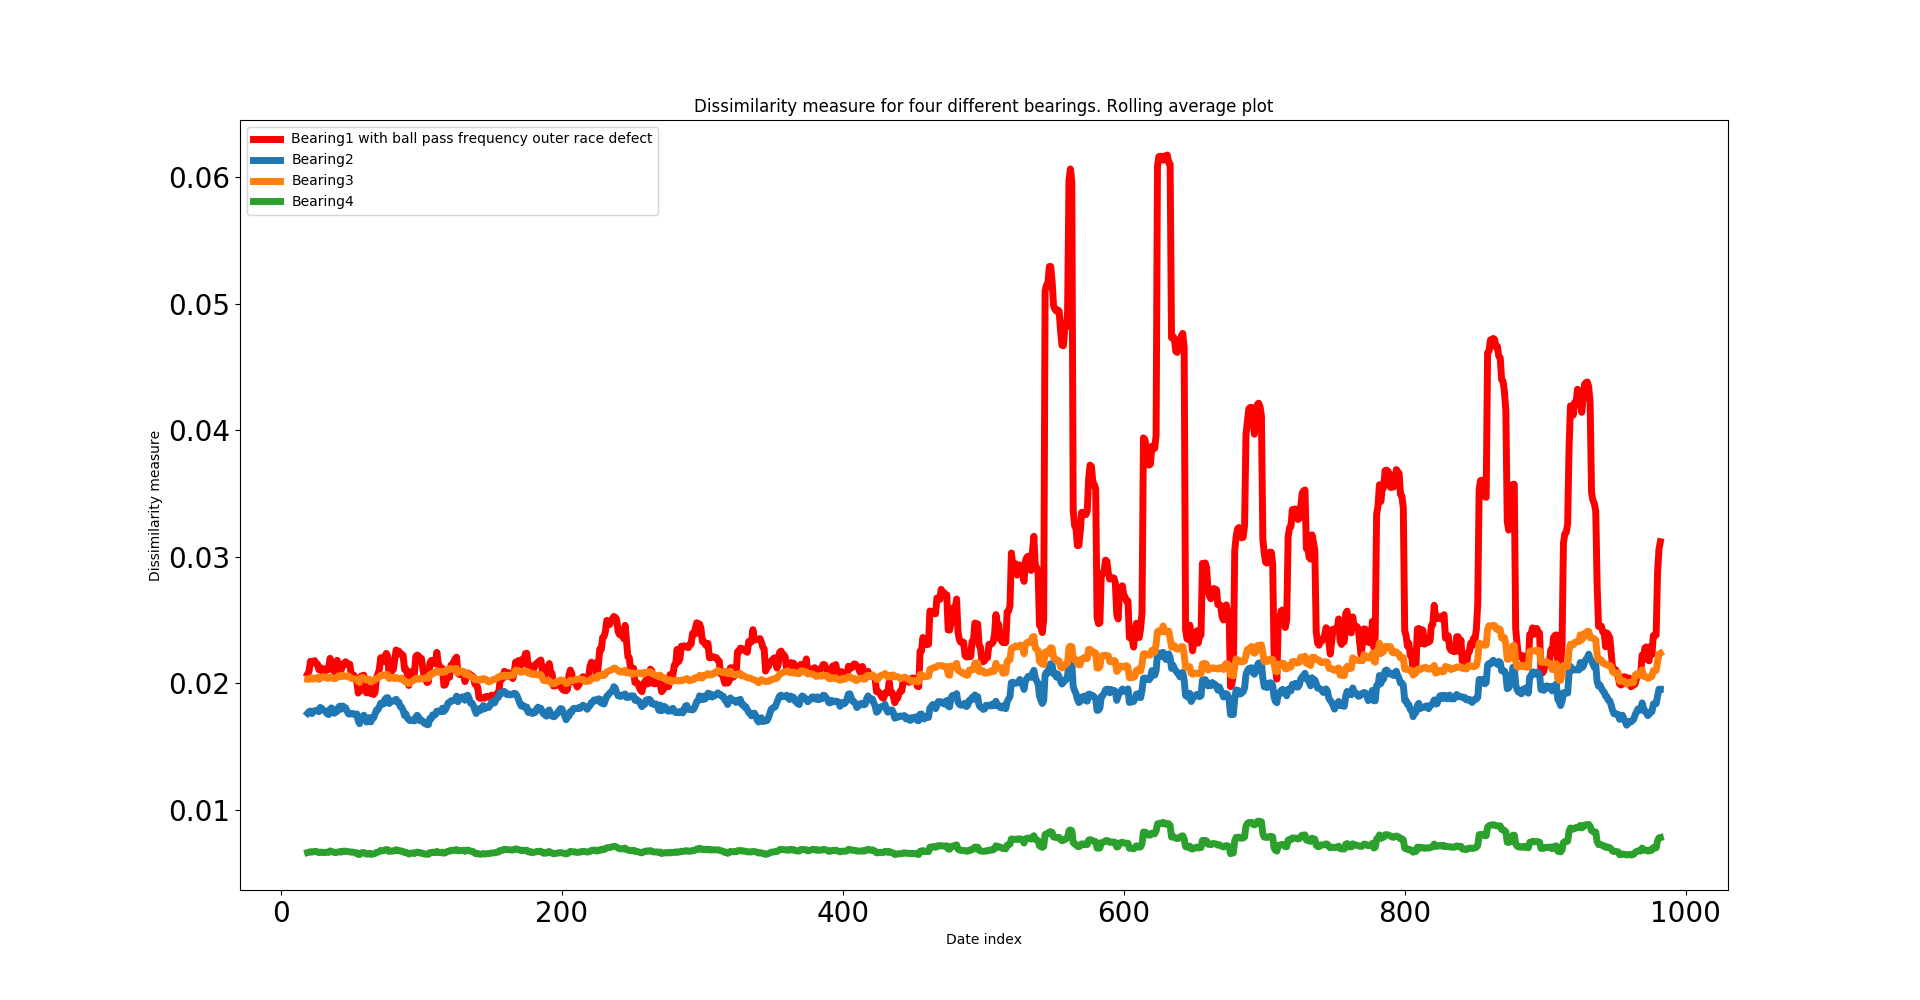
\includegraphics[width=7in]{statistics_dissimilarity_bpfo} 
   \caption{Dissimilarity measure for four bearings. In red a bearing with ball pass frequency outer race defect}
   \label{fig:example}
\end{figure}

\begin{figure}[H] %  figure placement: here, top, bottom, or page
   \centering
   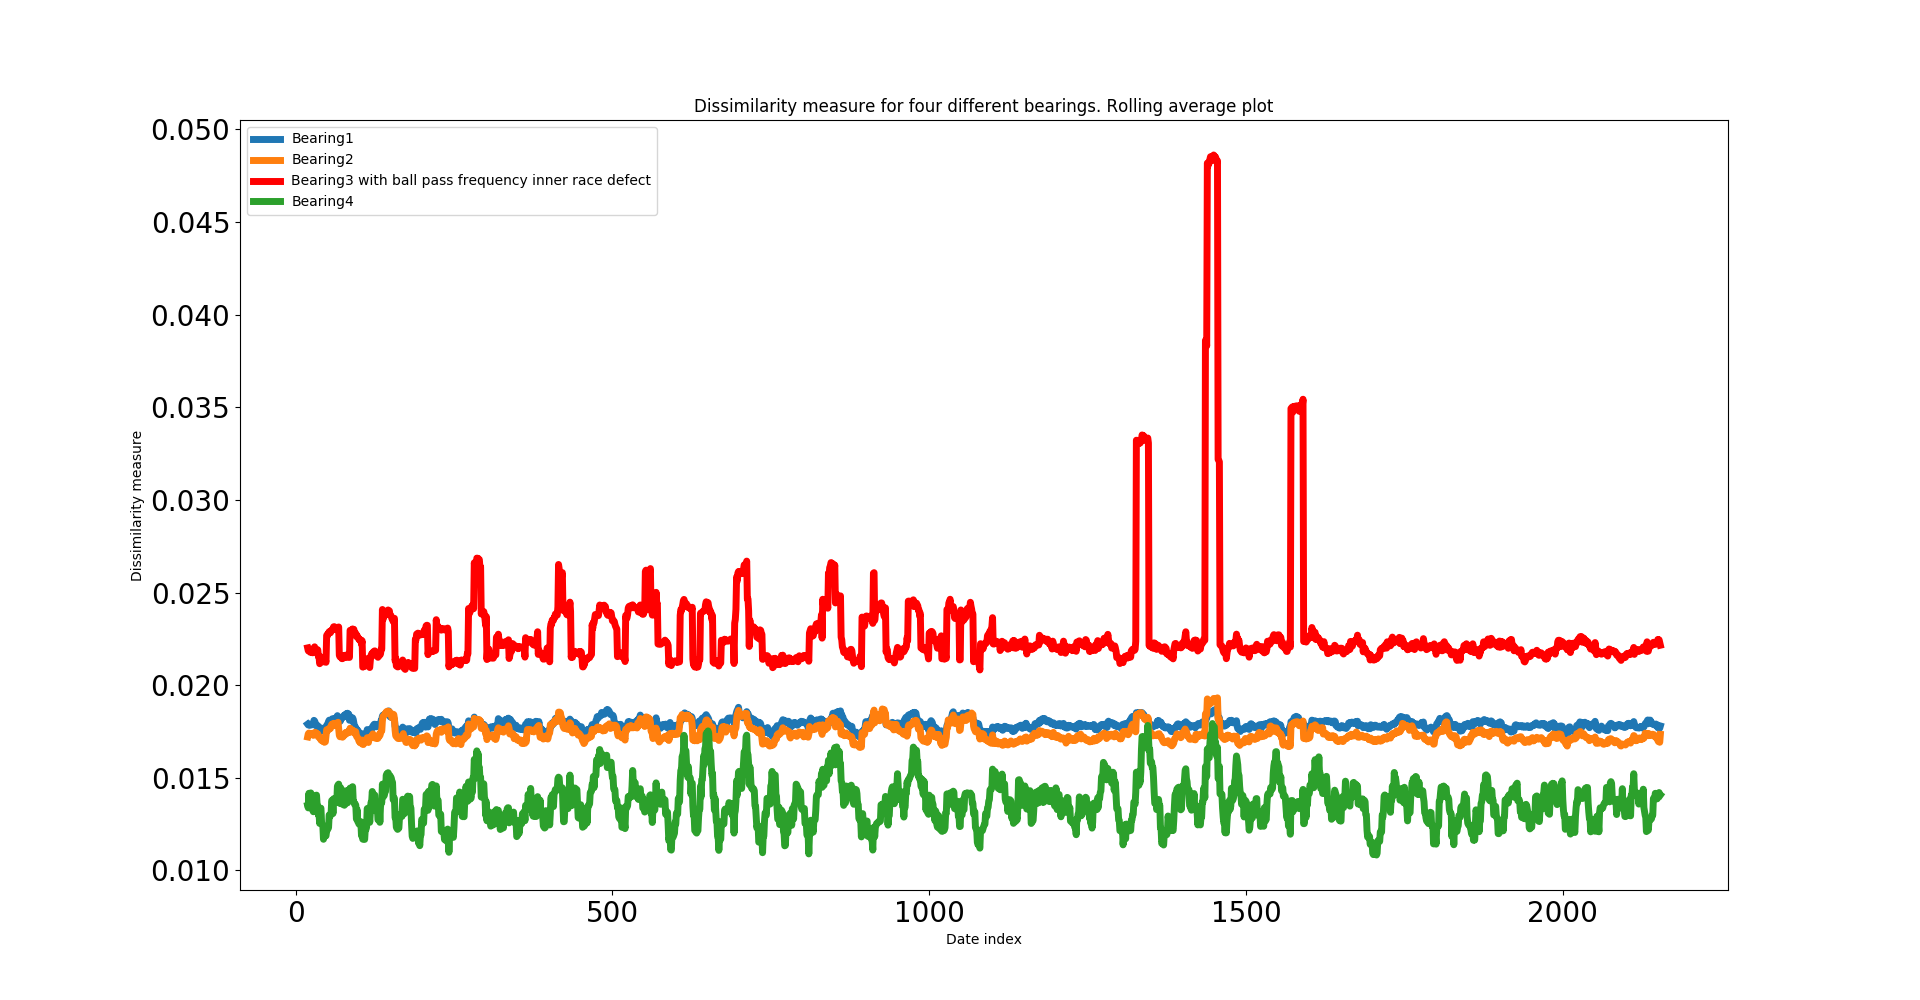
\includegraphics[width=7in]{statistics_dissimilarity_bpfi} 
   \caption{Dissimilarity measure for four bearings. In red a bearing with ball pass frequency inner race defect}
   \label{fig:example}
\end{figure}

As we can see on the above figures, the bearings with outer race and inner race defect have the highest dissimilarity measure. The dissimilarity measures quantifies the health index of a bearing. A higher dissimilarity implies bearing degradation.
%%%%%%%%%%%%%%%%%%%%%%%%%%%%%%%%%%%%%%%%%%%%%%%%%%%%%%%%%%%%%%%%%%%%%%%%%%%%%%%%%%%%
%%%%%%%%%%%%%%%%%%%%%%%%%%%%%%%%%%%%%%%%%%%%%%%%%%%%%%%%%%%%%%%%%%%%%%%%%%%%%%%%%%%%
%%%%%%%%%%%%%%%%%%%%%%%%%%%%%%%%%%%%%%%%%%%%%%%%%%%%%%%%%%%%%%%%%%%%%%%%%%%%%%%%%%%%
\section{Mixed method: statistical and wavelet approach}
\begin{figure}[H] %  figure placement: here, top, bottom, or page
   \centering
   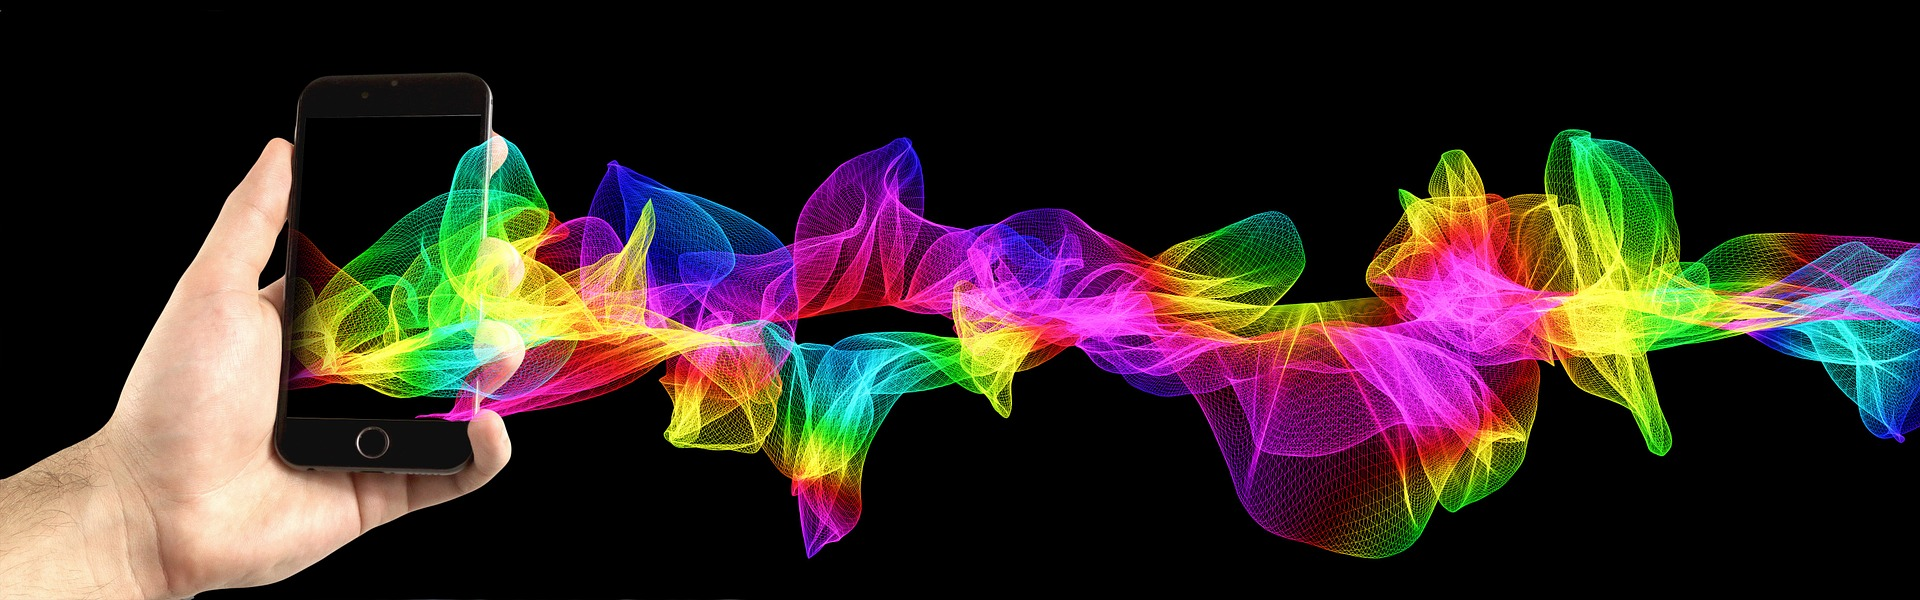
\includegraphics[width=4in]{mixed4} 
   \caption{}
   \label{fig:example}
\end{figure}
For the mixed method, we use wavelet transform to generate two extra features from the vibration time signal, namely the discrete detailed coefficient cD and the approximate coefficient cA. The detail coefficient cD represents the hight frequency component of the vibration time signal and the approximate coefficient cA represents  
the low frequency component.  For the mother wavelet we use Daubechies 20 or db20.

\begin{figure}[H] %  figure placement: here, top, bottom, or page
   \centering
   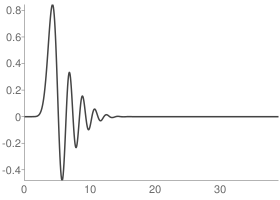
\includegraphics[width=2in]{dbscaling}
    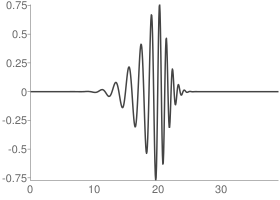
\includegraphics[width=2in]{dbwavelet}  
   \caption{The scaling function $\varphi$ (left) and the wavelet function $\Psi$ (right) }
   \label{fig:example}
\end{figure}

 A pseudo code in python to implement the method:
\begin{python}
pip install pywavelet
\end{python}
\begin{python}
import pywt
import numpy as np
container = []
mother_wavelet = 'db20'
ref_cA, ref_cD = pywt.dwt(ref_sample, mother_wavelet)
for sample in samples:
	cA, cD = pywt.dwt(ref_sample, mother_wavelet)
	cA_dissimilarity = dissimilarity_measure(ref_cA,cA)
	cD_dissimilarity = dissimilarity_measure(ref_cD,cD)
	container.append((cA_dissimilarity,cD_dissimilarity))
\end{python}
\begin{flushleft}
Once we have the two extra features, we compute the dissimilarity between a reference sample and subsequent samples for each feature. 
This process generates a set of points $(x,y)$ that represent the health index of each sample. As can be seen in the figure bellow, a bearing can go through three main stages:
\begin{enumerate}
\item A healthy stage characterised by a low health index
\item A warning stage characterised by an increasing health index
\item An alarm stage characterised by a high health index
\end{enumerate}

\end{flushleft}

K.C. Deekshit Kompella a, Venu Gopala Rao Mannam b, Srinivasa Rao Rayapudi
\begin{figure}[H] %  figure placement: here, top, bottom, or page
   \centering
   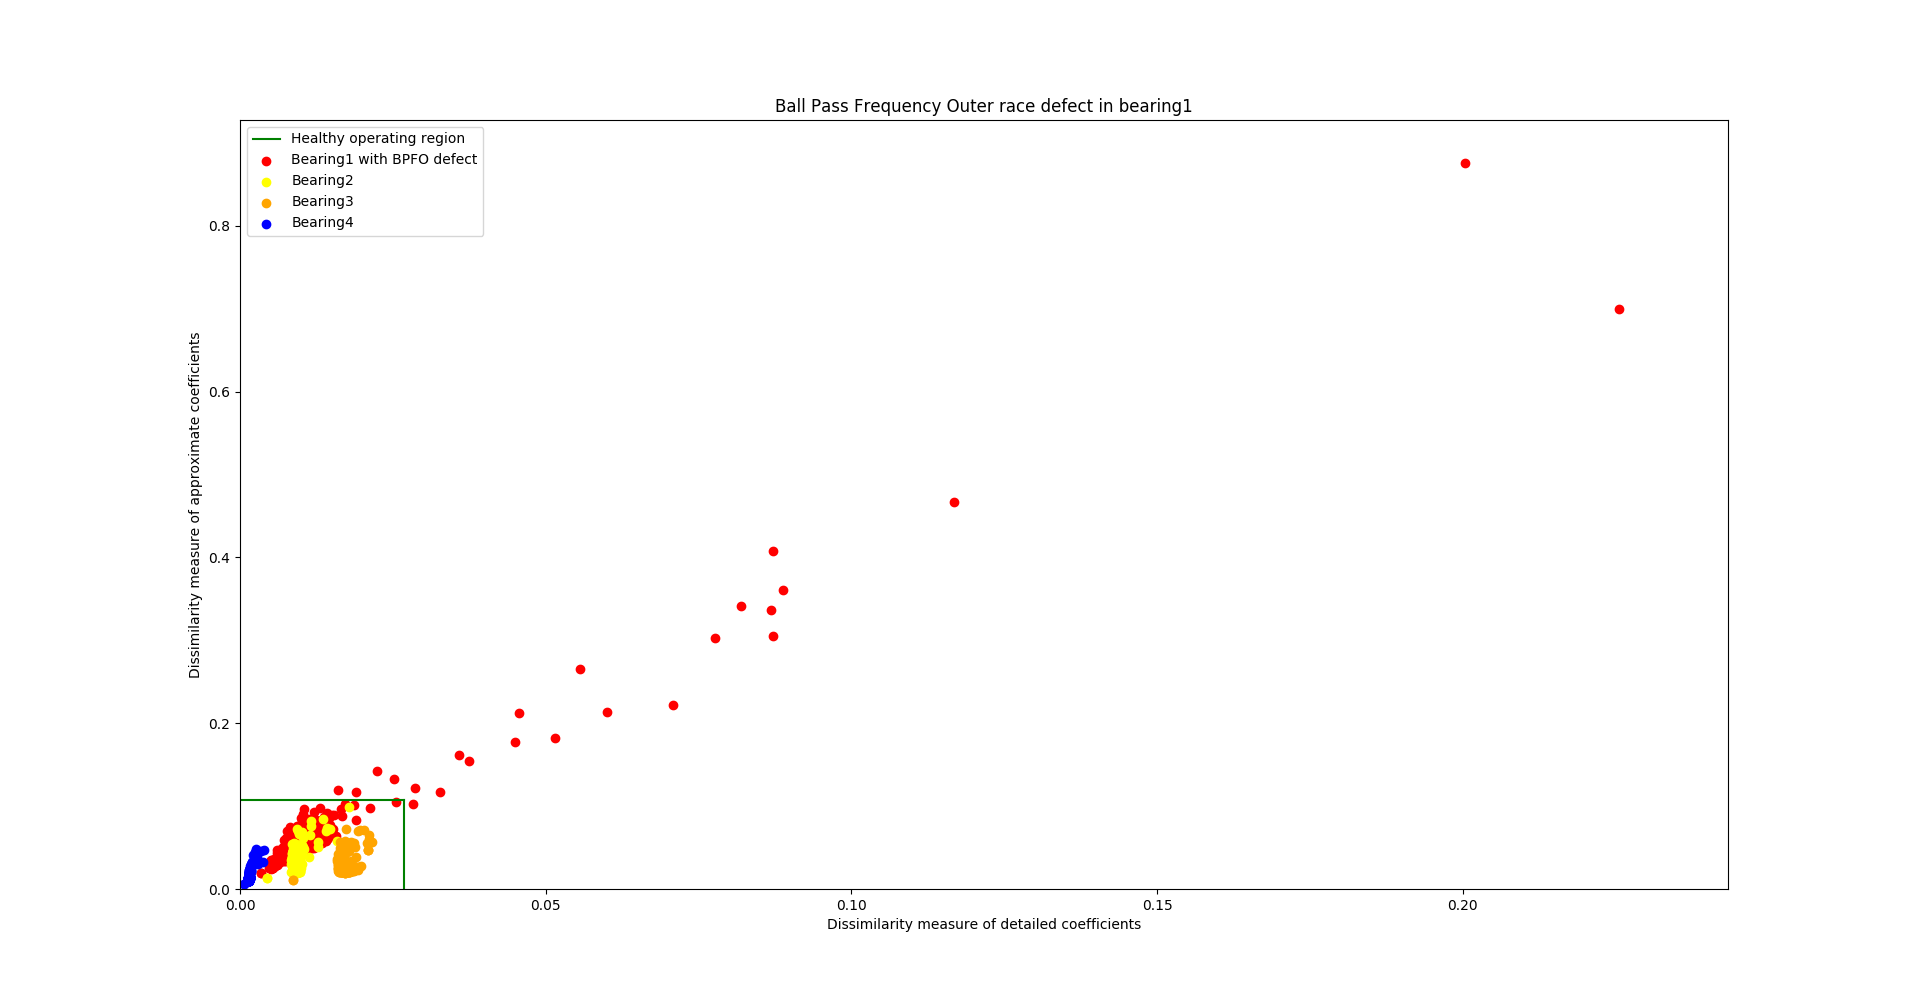
\includegraphics[width=6in]{mixed_method_bpfo.png} 
   \caption{}
   \label{fig:example}
\end{figure}
\begin{figure}[H] %  figure placement: here, top, bottom, or page
   \centering
   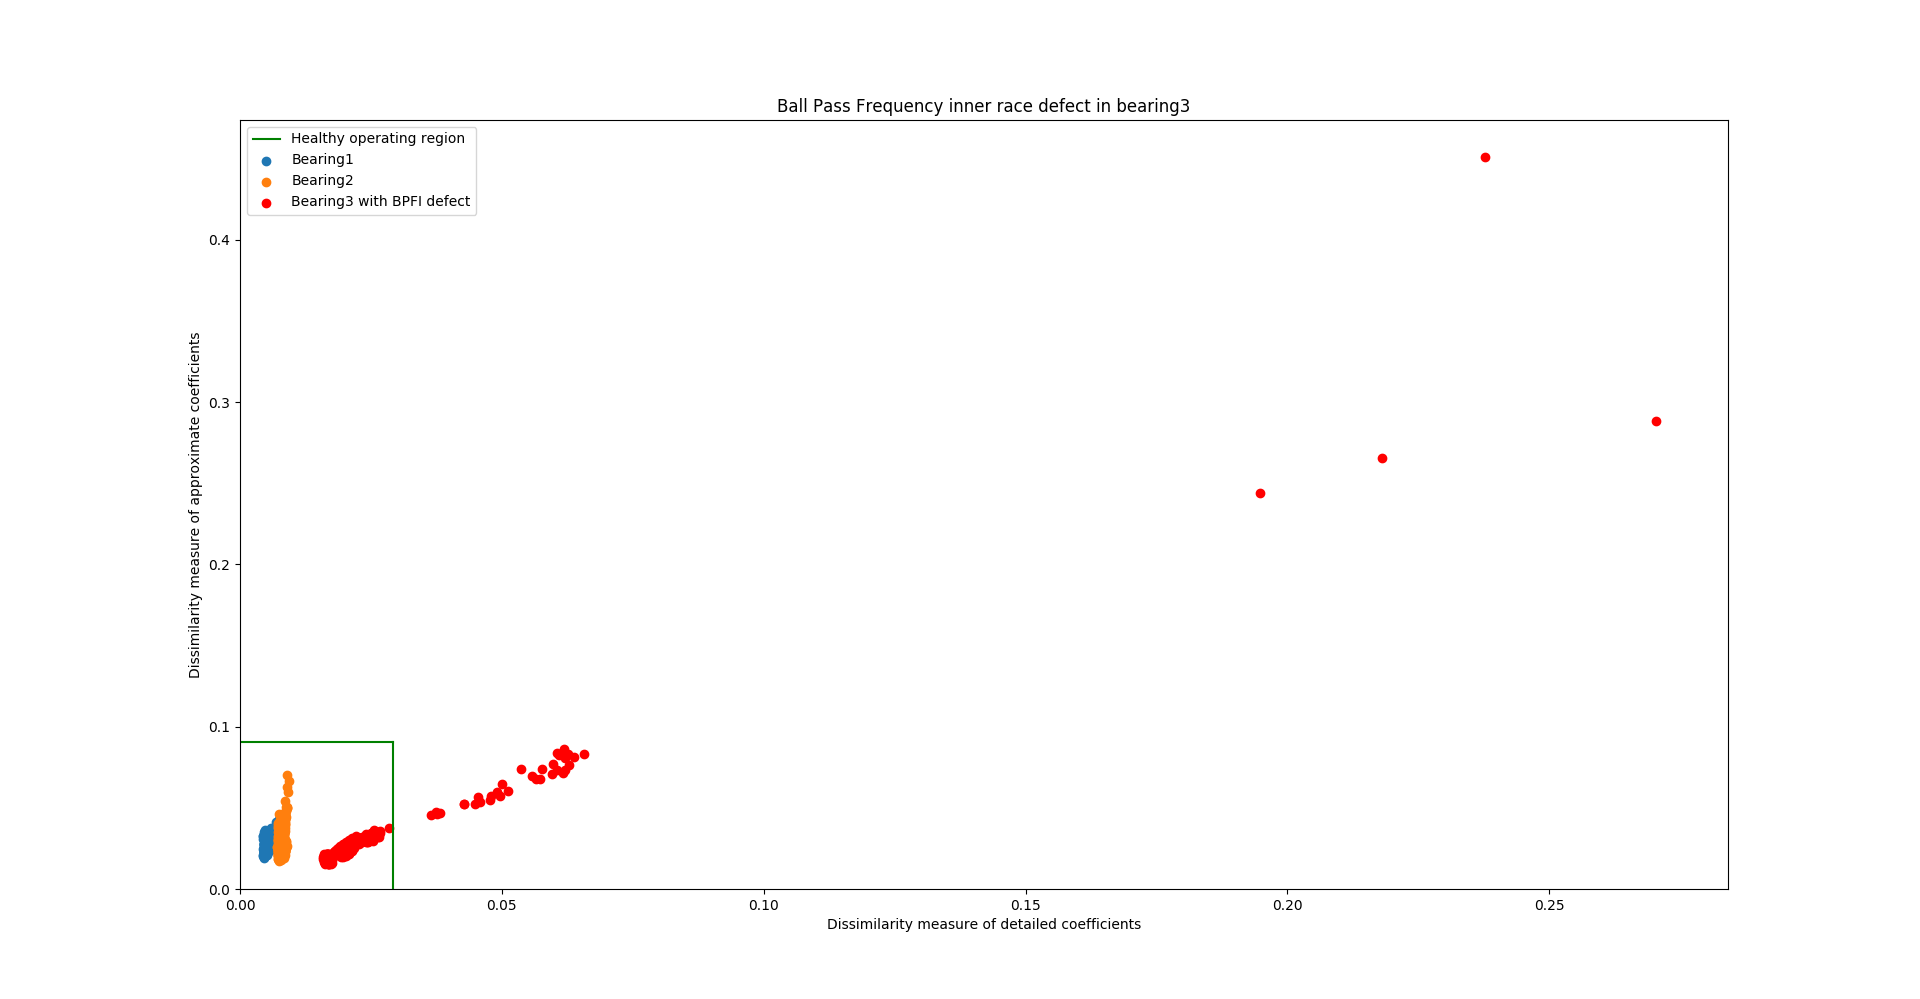
\includegraphics[width=6in]{mixed_method_bpfi.png} 
   \caption{}
   \label{fig:example}
\end{figure}
In the alarm stage, as the degradation becomes more severe, the distance between the points increases.
\section{Comparison}
The Signal processing method allows finding the nature or type of the fault and monitor the amplitude of the fault frequency. In the mixed method, we can only detect if there is fault but we cant specify for sure which kind of fault. The same goes for the mixed method. However in the mixed method we can estimate the time of failure based on the distance between the points formed by the dissimilarity of the detailed and approximate coefficients of the time signal wavelet transform.
\begin{flushleft}
The signal processing method relies on the RPM (the speed of the motor) to compute the fault frequency. If the RPM is inaccurate, it can be challenging to find a fault frequency. The statistical and mixed method only rely on the time signal.
\end{flushleft}



\end{document}  